

\section{Burgers' equation}

The inviscid Burgers' equation is the simplest {\em nonlinear} hyperbolic
equation:
\begin{equation}
u_t + u u_x = 0
\end{equation}
Here $u$ is both the quantity being advected and the speed at which 
it is moving.  Recall that for the linear advection equation, we saw
that the solution was constant along lines $x = ut + x_0$, which are
parallel, since $u$ is spatially constant.  For Burgers' equation, 
this is no longer the case, and the characteristic lines are now
given by $dx/dt = u$, with $x(0) = x_0$.  Since $u = u(t)$, we cannot
integrate this directly.   

If we take $u_0 = u(t=0)$, then we can look at how the characteristic
behave initially (before $u(x,t)$ changes a lot).
Figure~\ref{fig:burgers_char} shows the behavior of an initial
sinusoidal velocity.  We see that after a short period of time, the
characteristics intersect.  At the point, $(x_s, t_s)$ where they 
intersect, there is no way to trace backwards along the characteristics to
find a unique initial state.  This merging of the characteristics in 
the $x$-$t$ plane is a shock, and represents just one way that nonlinear
problems can differ from linear ones.

\begin{figure}[t]
\centering
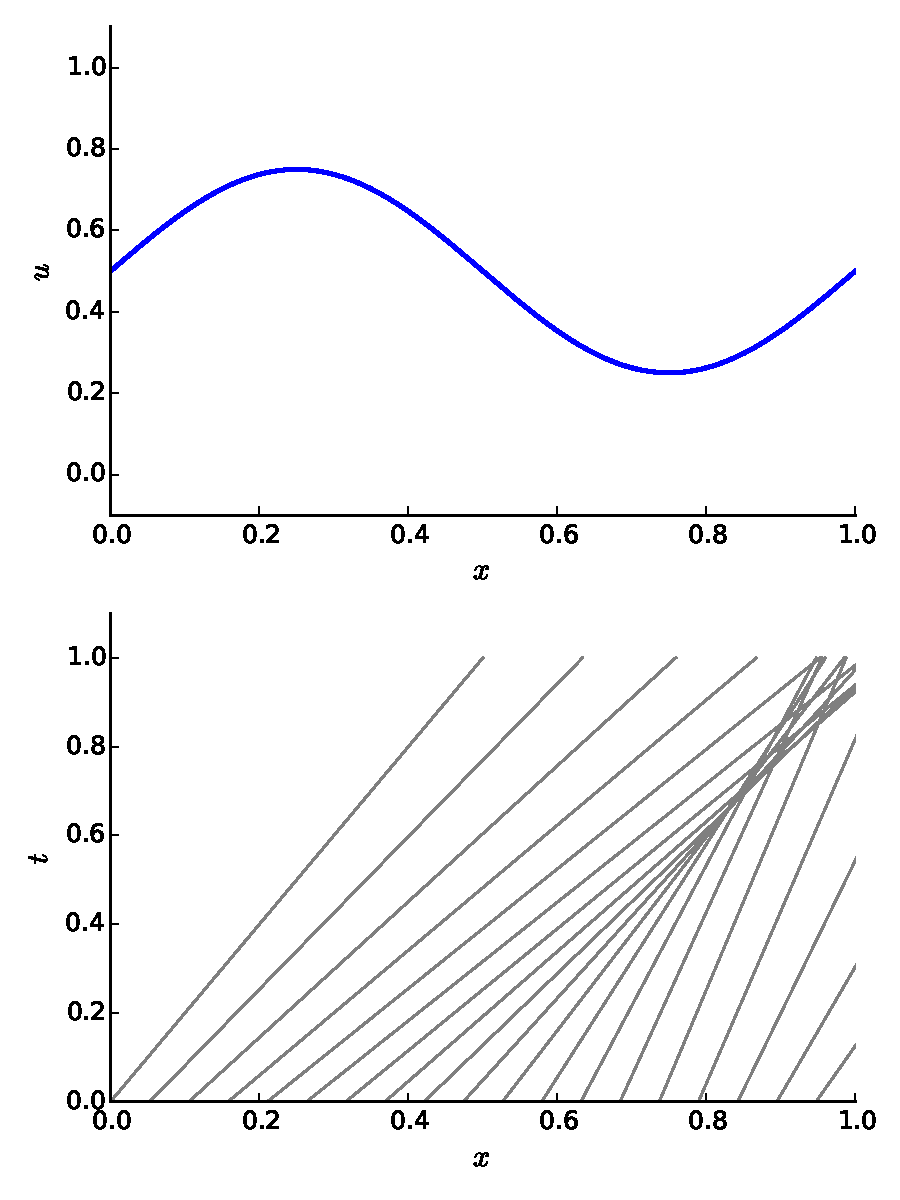
\includegraphics[width=0.6\linewidth]{burgers-characteristics}
\caption[Characteristics for shock initial conditions]
{\label{fig:burgers_char} (top) Initially sinusoidal
velocity distribution (bottom) Approximate characteristic
structure for Burgers' equation, using $u_0 = u(t)$.  Note that
after a short period of time, the characteristics intersect, signaling
the formation of a shock.}
\end{figure}



In conservative form, Burgers' equation appears as:
\begin{equation}
u_t + \left [\tfrac{1}{2} u^2 \right ]_x = 0
\end{equation}
The solution of this follows the same methodology as outlined above.
The interface states are predicted as:
\begin{eqnarray}
u^{n+1}_{i+1/2,L} 
 &=& u^n_i + \frac{\Delta x}{2} \frac{\partial u}{\partial x}
    + \frac{\Delta t}{2} \left . \frac{\partial u}{\partial t} \right |_i
    + \ldots \\
 &=& u^n_i + \frac{\Delta x}{2} \frac{\partial u}{\partial x}
    + \frac{\Delta t}{2} \left . \left (-u_i \frac{\partial u}{\partial x} 
         \right ) \right |_i 
    + \ldots \\
 &=& u^n_i + \frac{\Delta x}{2} 
   \left ( 1 - \frac{\Delta t}{\Delta x} u_i \right ) 
   \left . \frac{\partial u}{\partial x} \right |_i + \ldots
\end{eqnarray}
The only difference with the linear advection equation is that now
$u_i \Delta t/\Delta x$ varies from zone to zone, whereas with linear
advection, it is the constant $C$.  The slopes are computed using
the same limiters as with linear advection. 

The Riemann problem differs from linear advection.  As we saw above,
the characteristic curves can intersect in the $x$-$t$ plane, and it
is not possible to trace backward from time to learn where the flow
originated.  This is the condition for a {\em shock}.

\begin{figure}[t]
\centering
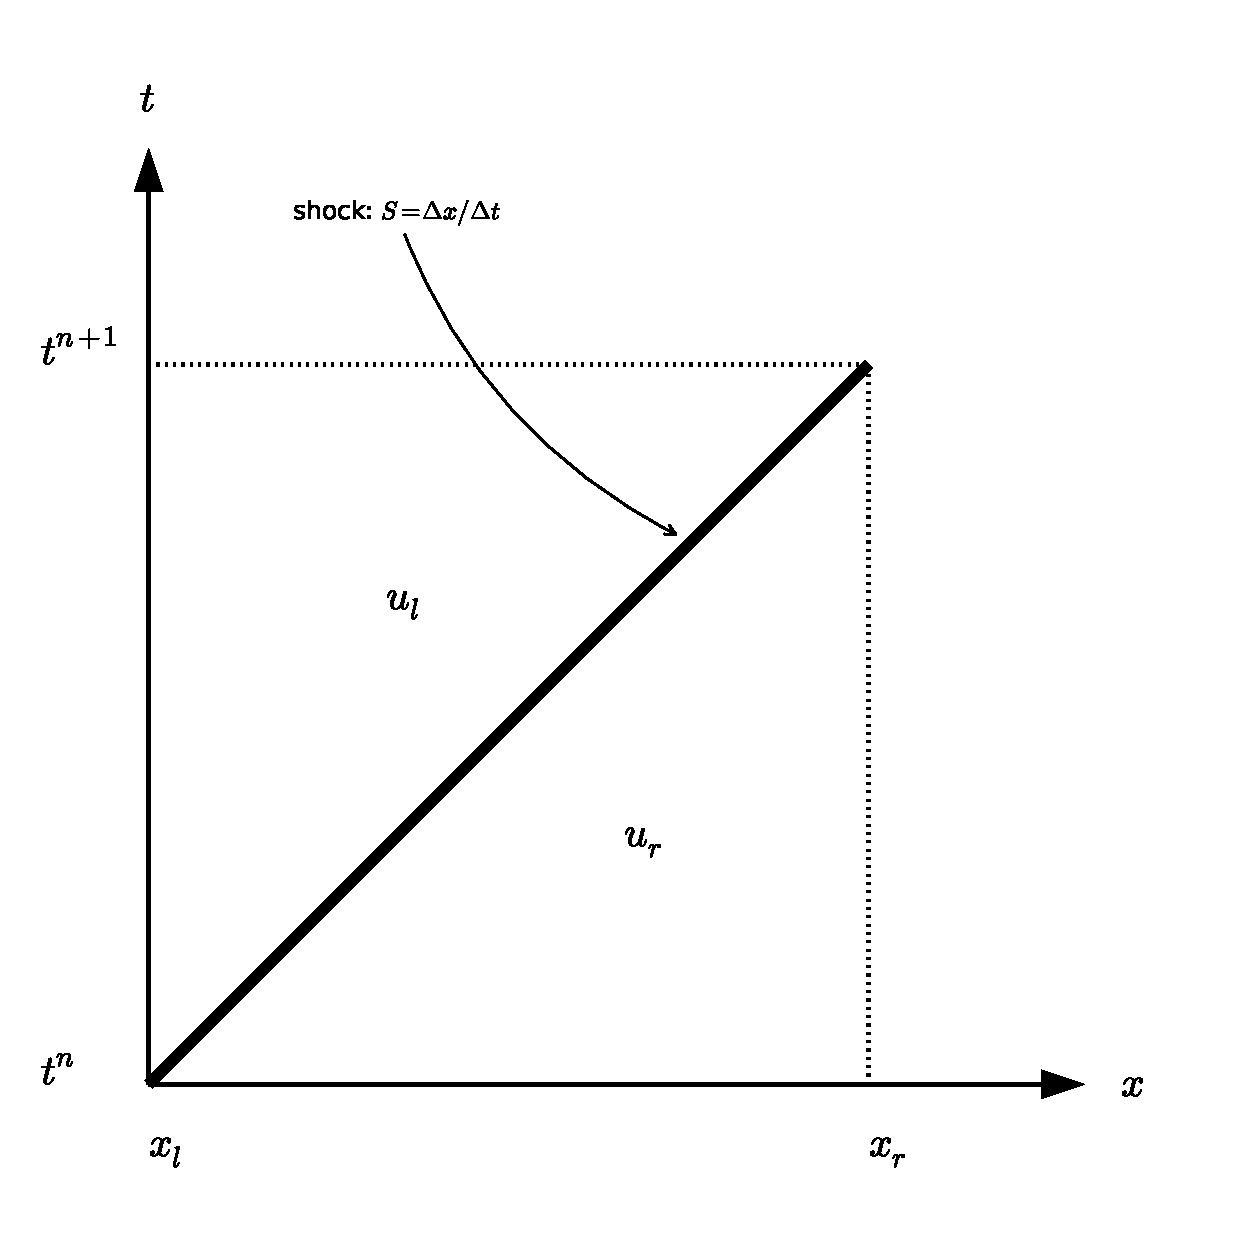
\includegraphics[width=4in]{rh}
\caption[Rankine-Hugoniot conditions]{\label{fig:rh} A rightward moving shock in the $x$-$t$
   plane separating two states: $u_l$ and $u_r$.}
\end{figure}

The shock speed is computed through the {\em Rankine-Hugoniot} jump
conditions.  For a scalar equation, these are easy to construct.
We'll follow the method of \cite{leveque:2002}.  Figure~\ref{fig:rh}
shows two states separated by a rightward moving shock in the $x$-$t$
plane.  At time $t^n$, the state in our interval ($x \in [x_l,x_r]$)
is entirely $u_r$.  As time evolves, we imagine our interval $[x_l,x_r]$ moving
vertically upwards in the diagram, and we see that it contains a mix of states $u_l$ and $u_r$.  Finally, at time, $t^{n+1}$ it is entirely
$u_l$.  The shock moves with a speed $S = \Delta x/\Delta t$ in this
figure.  To determine the speed, we integrate our conservation law over
both space and time (and normalize by $\Delta x = x_r - x_l$):
\begin{equation}
\frac{1}{\Delta x} \int_{x_l}^{x_r} dx \int_{t^n}^{t^{n+1}} dt u_t = 
  - \frac{1}{\Delta x} \int_{x_l}^{x_r} dx \int_{t^n}^{t^{n+1}} dt \left [ f(u) \right ]_x
\end{equation}
Doing the $t$ integral on the left and $x$ integral on the right, we have
\begin{equation}
\frac{1}{\Delta x} \int_{x_l}^{x_r}\left \{ u(t^{n+1}) - u(t^n) \right \} dx = 
  - \frac{1}{\Delta x} \int_{t^n}^{t^{n+1}} \left \{ f(u) |_{x=x_r} - f(u) |_{x=x_l} \right \} dt
\end{equation}
Recognizing that at $t=t^n$, $u = u_r$ and at $t=t^{n+1}$, $u = u_l$,
$\{ u(t^{n+1}) - u(t^n) \}$ in the left side becomes $\{ u_l -u_r \}$.
For the right side, we see that all along $x=x_l$ the flux is $f =
f(u_l)$ for $t\in [t^n, t^{n+1}]$.  Likewise, all along $x=x_r$, the
flux is $f = f(u_r)$ in the same time interval (see the figure).
Therefore, our expression becomes:
\begin{equation}
(u_l - u_r) = -\frac{\Delta t}{\Delta x} \left [ f(u_r) - f(u_l)\right ]
\end{equation}
and using $S = \Delta x/\Delta t$, we see
\begin{equation}
S = \frac{f(u_r) - f(u_l)}{u_r - u_l}
\end{equation}

For Burgers' equation, substituting in $f(u) = u^2/2$, we get
\begin{equation}
S = \frac{1}{2}(u_l + u_r)
\end{equation}

With the shock speed known, the Riemann problem is straightforward.  If there
is a shock (compression, so $u_l > u_r$) then we compute the shock speed and
check whether the shock is moving to the left or right, and then use the appropriate
state.  If there is no shock, then we can simply use upwinding, as there is no
ambiguity as to how to trace backwards in time to the correct state.
Putting this together, we have:
\begin{eqnarray}
\mathrm{if~} \underset{\text{(shock)}}{u_l > u_r}:&& u_s = \left \{ \begin{array}{cl}
                u_l & \mathrm{if~} S > 0 \\ 
                u_r & \mathrm{if~} S < 0 \\
                0   & \mathrm{if~} S = 0 \end{array} \right .   \\[1em]
%
\mathrm{otherwise:}&& u_s = \left \{ \begin{array}{clc}
                u_l & \mathrm{if~} u_l > 0 \\  
                u_r & \mathrm{if~} u_r < 0 \\  
                0   & \mathrm{otherwise} \end{array} \right .   
\end{eqnarray}
               
Once the interface states are constructed, the flux is calculated as:
\begin{equation}
F^{n+1/2}_{i+1/2} = \frac{1}{2} \left (u_{i+1/2}^{n+1/2} \right )^2
\end{equation}
and the conservative update is
\begin{equation}
u_i^{n+1} = u_i^n + \frac{\Delta t}{\Delta x} 
   \left ( F_{i-1/2}^{n+1/2} - F_{i+1/2}^{n+1/2} \right )
\end{equation}

The timestep constraint now must consider the most restrictive Courant 
condition over all the zones:
\begin{equation}
\Delta t = \min_i \left \{ \Delta x / u_i \right \}
\end{equation}


\begin{figure}[t]
\centering
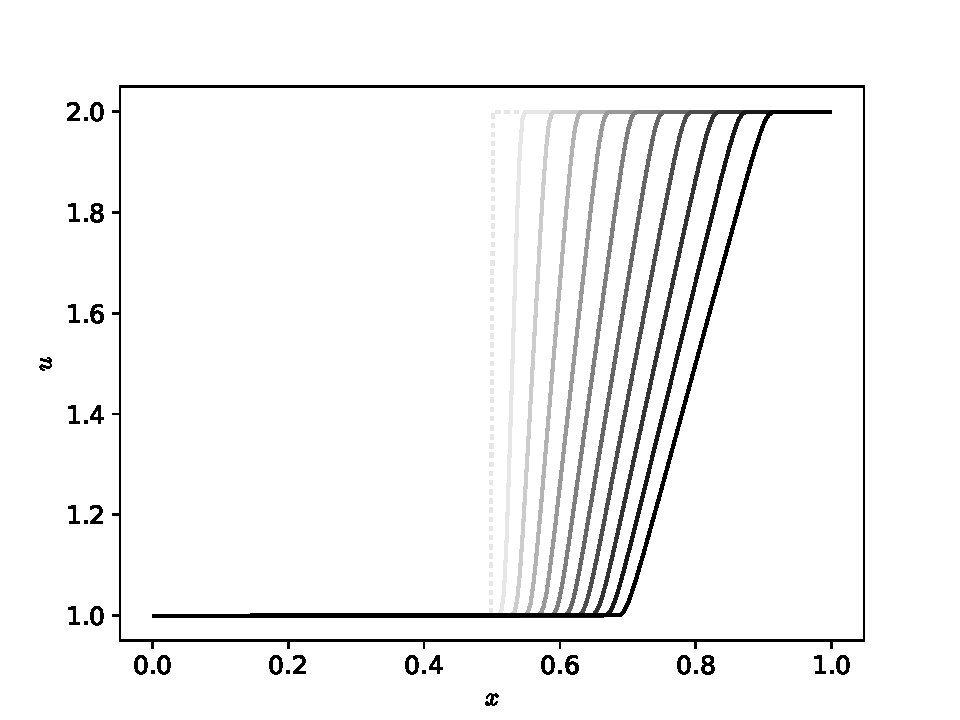
\includegraphics[width=0.8\linewidth]{fv-burger-rarefaction} 
\caption[Rarefaction solution to the inviscid Burgers'
  equation]{\label{fig:burgers-rarefaction} Solution to the inviscid
  Burgers' equation with 256 zones and a Courant number, $C = 0.8$ for
  initial conditions that generate a rarefaction: the left half of the
  domain was initialized with $u = 1$ and the right half with $u = 2$.
  This initial velocity state creates a divergent flow.  The curves
  are shown 0.02~s apart, with the darker grayscale representing later
  in
  time. \\ \hydroexdoit{\href{https://github.com/zingale/hydro_examples/blob/master/burgers/burgers.py}{burgers.py}}}
\end{figure}


Figure~\ref{fig:burgers-rarefaction} shows the solution to Burgers'
equation using the 2nd-order piecewise linear method described here,
with the MC limiter.  The initial conditions chosen are all positive
velocity, with a lower velocity to the left of the higher velocity.
As the solution evolves, the state on the right will rush away from
the state on the left, and spread out like a fan.  This is called a
{\em rarefaction wave} or simply a {\em rarefaction}.

\begin{figure}[t]
\centering
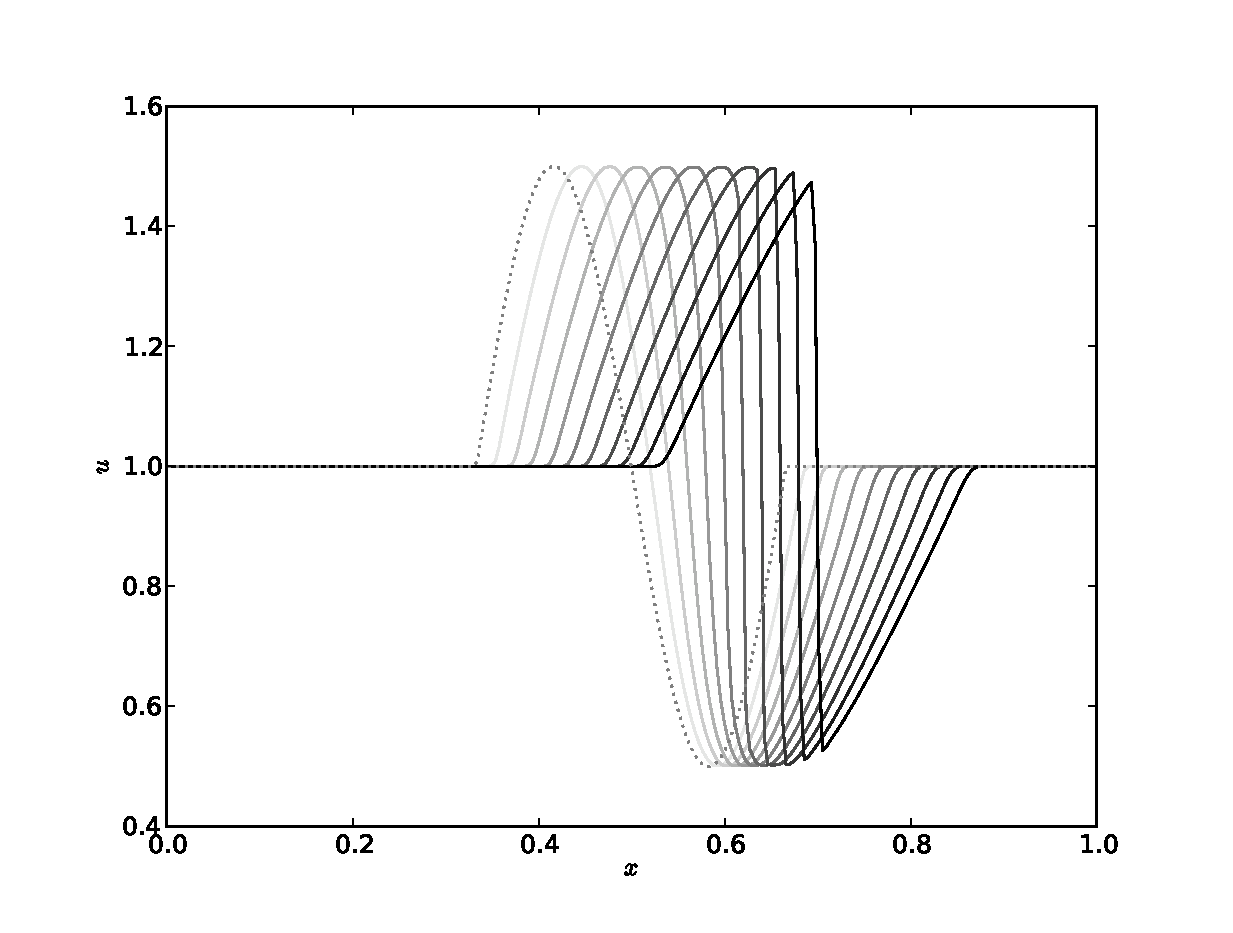
\includegraphics[width=0.8\linewidth]{fv-burger-sine}
\caption[Shock solutions to the inviscid Burgers'
  equation]{\label{fig:burgers-shock} Solution to the inviscid
  Burgers' equation with 256 zones and a Courant number, $C = 0.8$.
  The initial conditions here are sinusoidal and the solution quickly
  steepens into a shock.The curves are shown 0.02~s apart, with the
  darker grayscale representing later in
  time. \\ \hydroexdoit{\href{https://github.com/zingale/hydro_examples/blob/master/burgers/burgers.py}{burgers.py}}}
\end{figure}

Figure~\ref{fig:burgers-shock} shows the solution to Burgers'
equation with initially sinusoidal data:
\begin{equation}
\renewcommand{\arraystretch}{1.75}
u(x, t=0) = \left \{ \begin{array}{cc}
    1   & x < 1/3 \\
    1 + \frac{1}{2} \sin\left (\frac{2\pi (x - 1/3)}{1/3}\right ) & 1/3 \le x \le 2/3 \\
    1   & x > 2/3 
\end{array}
\right .
\renewcommand{\arraystretch}{1.0}
\end{equation}
This is analogous to the case shown in
Figure~\ref{fig:burgers_char}---we see the solution steepen and form a
shock which propagates to the right.  The shock is practically infinitesimally thin
here, since there is no explicitly viscosity to smear it out\footnote{Numerical diffusion,
in the form of truncation error of our method, will smear things a little.}.

\begin{exercise}[Simple Burgers' solver]
{Extend your 1-d finite-volume solver for advection (from
  Exercise~\ref{adv:ex:fv}) to solver Burgers' equation.  You will
  need to change the Riemann solver and use the local velocity in the
  construction of the interface states.  Run the examples shown in
  Figures~\ref{fig:burgers-rarefaction} and \ref{fig:burgers-shock}}.
\end{exercise}

As we'll see shortly, these two types of waves can also appear in the Euler equations
for hydrodynamics.

A final thing to note is that we solved Burgers' equation in conservative form.
For shock solutions, this is essential, since as we noted earlier, that finite-volume
method relates to the integral form of the PDEs, the discontinuity is nicely handled
by the Riemann solver.  We could also imagine differencing Burgers' equation in
non-conservative form, i.e., starting with:
\begin{equation}
u_t + u u_x = 0
\end{equation}
If you did this (for instance, using a finite difference scheme and an
upwind difference for $u_x$), you would find that you get the wrong
shock speed.  Try it.


\section{Characteristic tracing}

A concept that will be useful in the next section is {\em
  characteristic tracing}.  The idea is that we only include
information in the interface states if the characteristic that carries
that information is moving toward the interface.  For Burgers equation,
this is simple, since there is only a single characteristic---the velocity.
So for the left state on an interface, we'd only add the change if 
the velocity $u_i > 0$ (moving toward the interface $i+1/2$):
\begin{equation}
u^{n+1}_{i+1/2,L} 
 = u^n_i + \frac{\Delta x}{2} 
   \left ( 1 - \frac{\Delta t}{\Delta x} \max(0, u_i) \right ) 
   \left . \frac{\partial u}{\partial x} \right |_i + \ldots
\end{equation}
Notice that the effect of this is to set the interface state simply to
the value given by the piecewise linear reconstruction on the interface
if the wave isn't moving to the interface.  

\section{Going further}

\begin{itemize}
\item The equation we've been dealing with here is the {\em inviscid} Burgers' equation. 
The full Burgers' equation includes viscosity (a velocity diffusion):
\begin{equation}
u_t + u u_x = \epsilon u_{xx}
\end{equation}
To solve this, we need to first learn about techniques for diffusion, and then how to
solve equations that span multiple PDE types.  This will be described in \S \ref{ch:multiphysics:sec:adburgers}.

\item Aside from pedagogical interest, Burgers' equation can be used as a simple
model of traffic flow (where shocks can arise from people slamming on the brakes).
Many sources discuss this application, including the text by~\cite{leveque:2002}.

\end{itemize}
